\chapter{Software system modularity} \label{chapter3}
\minitoc
\eject

\section{Introduction}

In this thesis, we are interested in the evolution of the development of web applications, constrained by an economical context.
In this chapter, we present a broader view on the development of software systems.
We present different fields of work related to ours, to finally refine the scope of our research on the subject of our interest.

% \cit{It is becoming increasingly important to the data-processing industry to be able to produce more programming systems and produce them with fewer errors, at a faster rate, and in a way that modifications can be accomplished easily and quickly.}{W. P. Stevens, G. J. Myers, L. L. Constantine \cite{Stevens1974}}.

Since the beginning of the software development discipline, the best practices advocate to organize the code into independent units.
It was called modular programming\cite{Parnas1972}, structured design\cite{Stevens1974}, hierarchical structure\cite{Dijkstra1968}, object-oriented programming among other names.
Each of these names represent slightly different approaches on the construction and composition of these units.
One recurring principle, though, is that the units are to be as loosely coupled as possible.
We are going to explain these approaches focused on improving the maintainability, and the growth of the software.

% http://userpage.fu-berlin.de/~ram/pub/pub_jf47ht81Ht/doc_kay_oop_en
% \textit{OOP to me means only messaging, local retention and protection and hiding of state-process, and extreme late-binding of all things. It can be done in Smalltalk and in LISP. There are possibly other systems in which this is possible, but I'm not aware of them.

% Cheers,

% Alan}

The focus of the software industry was to improve the development process.
The Moore's law\cite{Moore1965} assured an exponential evolution of the processing power, hence the execution speed was never to be a problem.
Until the clock speed of processors could not be increased.
The increasing number of transistors predicted by Moore's law were to be reorganized as several execution units into the same processor.

With multiple execution unit to coordinate, the decomposition of software system in modules have now two goals.
The growth of the software, as well as the decomposition of execution on the several execution units.
As Parnas famously showed in 1972\cite{Parnas1972}, these two approaches to decomposition are incompatible.
It seems impossible to develop a software following a decomposition that satisfies both the growth, and an efficient parallel execution. \nt{TODO more on that}

With the incentive to leverage the execution power of parallel architecture, many work followed aimed at providing tools and model to organize the execution on multiple execution units.
For example distributed systems, single instruction multiple data, among others.\nt{TODO not really good examples}

There has been many attempts at reconciling the two approaches.
But none seems really convincing enough to be widely adopted.
Throughout this chapter, I will classify different works from the community in one of these three category : focus on development growth, focus on parallel execution, or reconciliation of the two.

My objective in this thesis, as previously stated, is to find an equivalence between these two approaches in the case of streaming web applications.


\section{Development growth}

TODO introduction

\subsection{Modularity}

TODO introduction

\subsubsection{Structured Programming}

In the history of software development, at some point the size and complexity of software system urges the developers to split the problem into isolated subproblems.
Dijkstra was maybe the first to encounter and formalize this procedure.

A program expressed as a suites of instructions with occasional jumps makes the flow of control very hard to follow and understand.
We say it is spaghetti code.
Instead, Dijkstra advocated to forbid the use of the \texttt{goto} statement, and decompose the implementation into functions to be called and returned \cite{Dijkstra1968a}.
This would allow to split the main problem into many subproblems encapsulated into reusable, and isolated functions.
This is called structured programming, and it impacts the development at a fine grain by restricting the usage of the control flow.

Following this, he proposed to design complex systems with a hierarchical structure \cite{Dijkstra1968}.
Each layer would abstract a design problem for the upper layers.
This work established grounds for what is know called modular programming.

% Letters to the editor : goto statement considered harmful \cite{Dijkstra1968a}
% The structure of the THE-multiprogramming system \cite{Dijkstra1968}

\subsubsection{Structured Design}

Modular programming advocates to design a software system as an ensemble of modules communicating with each other.
When designing the modules, two properties are crucial, coupling and cohesion \cite{Stevens1974}.

The coupling defines the strength of the interdependence between modules.
It is opposed as cohesion which defines how strongly the features inside a module are related.
Low coupling between modules and high cohesion inside modules implies a better understanding and readability of the source code of the system.

The relations between features, necessary to define the module organization, needs to be well defined.
These relation will define the boundary of modules, and how the features should be put in those modules.


% (See wikipedia page https://en.wikipedia.org/wiki/Separation_of_concerns)


\subsection{Design choices}

TODO introduction

\subsubsection{Separation of concerns}

Dijkstra \cite{Dijkstra1982} coined the terms separation of concerns more than thirty years ago, but this concept drifted and loosed its initial meaning.
It is interesting to note the difference between the two meanings.
Initially, the separation of concerns meant the ability to reason about different properties of a software system.
My understanding of this definition, was not to encapsulate different concerns into different modules, but to analyze how a system possesses certain properties.
Dijkstra gives the example of analyzing correctness and efficiency independently.
In this respect, this thesis is completely oriented towards separating the concern of development maintainability and the concern of performance.
That is to be able to reason on the maintainability of a program, independently than of its performance, and vice versa.

However, separation of concerns seems rightfully to mean a different concept \cite{Tarr1999,Hursch1995}.
Separation of concerns is now understood as a design principle advocating that each module has a specific concern in a modular design.
For example, the separation of the form and the content in Latex, or in HTML / CSS are example of this new meaning for separation of concerns.

The drift in meaning seems to come from a confusion between a concern one have about this system, which is a property of the system (efficiency, readability, correctness), and a design choice to encapsulate to avoid impacting the whole system.

\subsubsection{Information hiding principle}

To my understanding, the new meaning of Separation of Concerns feels similar to the definition of information hiding.

Information hiding was defined by Parnas \cite{Parnas1972} as a way to define the organization of modules.
The intention was to encapsulate specific design choice in each module so as to limit the impact of the modification of a choice on the rest of the system.

In this article, Parnas clearly oppose the definition of modules following the flow of data through the execution, and the definition of modules following the information hiding principle.
In this thesis, we shall investigate further this opposition.



\subsection{Programming models}

TODO introduction

\subsubsection{Object oriented programming}

The following list define Object-Oriented Programming (OOP).

\begin{enumerate}
\item Everything is an object.
\item Communication is performed by objects communicating with each other, requesting that objects perform actions. Objects communicate by sending and receiving messages. A message is a request for action, bundled with whatever objects may be necessary to complete the task.
\item Objects have their own memory, which consists of other objects.
\item Every object is an instance of a class. A class simply represents a grouping of similar objects, such as integers or lists.
\item The class is the repository for behavior associated with an object. That is, all objects that are instances of the same class can perform the same actions.
\end{enumerate}

Though the recent concept of Object-oriented programming focus strongly on the notion of object as an encapsulation principle, Alan Kay who coined the term, insisted in a public mail exchange that the original concept he envisioned is about message-passing, more than inheritance.

Interestingly enough, Object Oriented Programming, as defined by Alan Kay, who coined the term, is based on the definition of the Actor Model.



\paragraph{Object calisthenics}

Object calisthenics are defined as the chapter 6 of \cite{Bay2008}.
It is an exercise presented as a list of 9 rules to follow to enforce maintainability and readability of your code.

Some of these rules are direct implementations of the more general concept of separation of concerns, and information hiding.
Rule 7 Keep all entities small, for example is similar somehow to say that entities should have a clear concern.
Other rules are just plain syntactic rules to improve readability and comprehensibility.


See Object calisthenics 
- http://williamdurand.fr/2013/06/03/object-calisthenics/
- http://www.cs.helsinki.fi/u/luontola/tdd-2009/ext/ObjectCalisthenics.pdf



\subsubsection{Another programming model ?}

TODO



\endinput







Plan

A first part with the modularity, from Parnas with Information Hiding, to modularity, and design decision, and design structure matrix, and so on ...
To Object, with object calisthenics.
This part should show roughly the trend in software modularity.

A second part with the incompatibility between this modularity and parallelism.
This part might need to move into the reconciliation part.






\subsubsection{Information Hiding Principles}

Reference paper :
On the criteria to be used in decomposing systems into modules \cite{Parnas1972}


The structure and value of modularity in software design \cite{Sullivan2001a}
-> We identify an issue for software designers that neither Parnas’s formulation nor subsequent developments based on it adequately address: A designer is responsible for producing the greatest benefit for any given investment of time, talent, money, and other resources.


\subsubsection{Modularity based on Design Decisions}

Designing Software for ease of extension and contraction \cite{Parnas1979}

Design Rules: The Power of Modularity Volume 1 \cite{Baldwin1999}
A reference book, but can't get it.

Design Rule Hierarchies and Parallelism in Software Development Tasks \cite{Wong2009}
Organize design, so that modules can be developed in parallel, without communication between teams working on independent modules.
Identification of coordination requirements \cite{Cataldo2006}
About the communication requirement between teams working on different modules.

If the teams working on different modules need not to communicate, then the same person working on different modules at different times, need not to remember any dependencies : both conserves locality of reasoning.


\subsubsection{Locality}

The Software Principle of Locality \cite{Dobson}
Not a very good article, but advocate principle of locality :
the person working closely, in terms of both space and time, to an artefact is the most qualified person to remove defects associated with it. This















\subsubsection{Contradiction}


To understand the problem of incompatibility between the modular design and the parallel execution, one can think about the communication between two stages.
The result output by one stage needs to be understood by the next.
There need to be a common understanding on the nature, and the structure of this result.
The modular design advocates that this common ground, the interface, be the most immutable possible, the most solid possible.
While the parallel execution defines interfaces between the stages.



\endinput

Since the beginning of software development, software systems are designed as the composition of smaller subsystems.\nt{Find exact reference of this}

The first one follows the Information Hiding principle, firstly stated by Parnas, in 1972 in his paper On the criteria to be used in decomposing systems into modules.

Dijkstra coined the term hierarchical structure in a paper presenting the decomposition of a multiprogramming system.
Basically what we could consider a simple operating system.

This paper also presents the what seems to be the very first concept of mutual exclusion, what is now regarded as an extremely difficult concept to master in concurrent programming.

In 2009 we can cite Wong, Design Rule Hierarchies and Parallelism in Software Development Tasks, that aim at improving the parallelism in development tasks.


But I am sure there is a lot more to find.
\begin{itemize}
  \item Structured Programming
  \item Hierarchical structure
  \item OOP
\end{itemize}





\endinput


Making state explicit for imperative big data processing \cite{Fernandez2014a}

Prospect: Finding and Exploiting Parallelism in a Productivity Language for Scientific Computing
http://2015.splashcon.org/event/splash2015-splash-i-lindsey-kuper-talk

Where is software headed ? \cite{Lewis1995}
-> Comparison between academic and industrial roadmap for software.

Now every programming languages use pass-by-reference, or pass-by-sharing to make use of the common memory storage.
Developers were always comfortable with this kind of storage abstraction.
It made sequential programming almost as efficient, and sometimes more, than parallel programming because of the optimization on sequential programming, and the difficulty and the lack of optimization of parallel programming.



I need to show that the 1) languages the more used are sequential with a common memory storage, because 2) it is inherently difficult to program with distributed memory storage.
3) I need to show that the best practice of software development require this common memory storage.

See Object calisthenics 
- http://williamdurand.fr/2013/06/03/object-calisthenics/
- http://www.cs.helsinki.fi/u/luontola/tdd-2009/ext/ObjectCalisthenics.pdf
\section{Parallel execution}


\subsection{Concurrency Theory}

The first models of computation, like the Turing machine and lambda-calculus, were inherently sequential and based on a global state.
As computers eventually evolved to become concurrent, a formalism was lacking  to represent concurrent computations.
The works on these models first tackled the problems of determinacy, communication and state synchronization.

We identify three main formal models for concurrent computations.
The Actor Model of C. Hewitt, the Pi-calculus of R. Milner and the Communicating Sequential Processes of T. Hoare.
Because these models represent a ground for all following work on concurrent programming, we briefly explain them in the next paragraphs.
These formalism have in common to state that input, output and concurrency should be regarded as primitives of programming.

% For more information, see : https://en.wikipedia.org/wiki/Actor_model_and_process_calculi_history

\subsubsection{Actor Model}

The Actor model allows to express the computation as a set of communicating actors \cite{Hewitt1973a, Hewitt1977, Clinger1981}.
In reaction to a received message, an actor can create actors, send messages, and choose how to respond to the next message.
All actors are executed concurrently, and communicate asynchronously.

The Actor model was presented as a highly parallel programming model, but intended for Artificial Intelligence purposes.
Its success spread way out of this first scope, and it became a general reference on message passing parallel programming.
For example, the Scala language advertises its use of an actor approach of concurrency.

% More recent work of C. Hewitt on Actors is about \nt{TODO} \cite{Hewitt2007,Hewitt2007a}.

The Actor model defined the message-passing communication paradigm.
The communication between two actors, the sender and the receiver, is a stream of discrete messages.
The sender names the receiver actor when sending messages to be the recipient of these messages.
Message-passing is often seen as asynchronous, because, contrary to the invocation, the sender doesn't wait for the result of the initiated communication. 

\subsubsection{Pi-calculus}

R. Milner presented a process calculus to describe concurrent computation : the Calculus of Communicating Systems (CCS) \cite{Milner1975, Milner1980}.
It is an algebraic notation to express identified processes communicating through labeled channels.
In CCS, process compose concurrently, communications are synchronous, and the topology is static.
The Pi-calculus improved upon this earlier work to allow processes to be communicated as values, hence to become mobile \cite{Engberg1986,Milner1992a,Milner1992}.
Contrary to CCS, in Pi-calculus processes can replicate and send process through channel, allowing dynamic modification of the topology.

Pi-calculus resembles to the actor model, but its algebraic nature led to a critical difference with the later.
Indeed, processes in the Pi-calculus communicate indirectly, through labeled ports, whereas actors communicate directly by naming the recipient actors.
This difference allows the same channel to lead to multiple processes in turns, whereas the recipient of a message cannot change. 
However, as the communication are synchronous, Pi-calculus cannot fully represent non-deterministic, hence real communications.
Moreover, Pi-calculus expresses concurrent computation, and not parallel computation, as progress can be made in only one process at a time.

% The pi-calculus led to Pict, a programming language\cite{Pierce2000}.

\subsubsection{Communicating Sequential Processes}

C. A. R. Hoare presented Communicating Sequential Processes (CSP) \cite{Hoare1978, Brookes1984}.
In CSP, processes are executed concurrently, and communicates events via channels.
The evolutions of this model were influenced by, and influenced the work of R. Milner, hence CCS and CSP are highly similar.
With the evolutions appeared the problems of determinism in distributed systems\nt{TODO}.\cite{Brookes1984}



\subsubsection{Concurrency, asynchronism and unbounded nondeterminacy}

All these early work adopted concurrent composition by default, instead of sequential composition, to adapt to the very concurrent nature of real parallel machines.
However, sequential programming is still the default.
Concurrent composition is yet still to be widely accepted, as stated by Reed \cite{Reed2012}.
\comment{TODO rewrite this paragraph}

All these works eventually evolved to adopt asynchronous communications.
Indeed, it is not realistic to build a distributed system based on synchronous communications. \nt{TODO reference needed}
By abandoning synchronous communication, such system also needs to abandon determinism.
It becomes non-deterministic because communications can take infinite time to complete.

Asynchronous communications are less expressive than synchronous ones \cite{PALAMIDESSI2003}.

\endinput



We need to wait a bit to see state synchronization outside of message-passing. \nt{TODO}




\subsection{Programming models}

To be read and added :

Distributed processes: a concurrent programming concept \cite{Hansen1978}

Monitors: an operating system structuring concept \cite{Hoare1974}

\subsubsection{Coroutines}

Conway defines coroutines as subroutines executing all at the same level.\cite{Conway1963}

\textit{A coroutine is an autonomous program which communicate with adjacent modules as if they were input and output subroutines.}

It defines the separability of a program, and advocates that coroutines be executed on separate processes, and communicate by sending discrete items.
This definition, is similar to that of actors.
The first definition of coroutine, explicitly specify that coroutines are best used when they can be executed, and communicate asynchronously.
However, most programming languages being synchronous, they then were implemented as synchronous routines, instead of independent processes.

Following work : Coroutines and Networks of Parallel Processes\cite{Kahn1976}

The coroutines defines the first pipeline organization of a program.

\subsubsection{Modules}

Multiprogramming designs the ability to program concurrent activities on multiple processing units.

Modula: A language for modular multiprogramming \cite{Wirth1977}

Modula is a descendent of Pascal with the addition of modules, that are essentially processes.


\subsubsection{Promises and Futures}

This \cite{Jr1977} is the reference paper for futures.

\subsubsection{Functional Reactive Programming}
\nt{I don't know exactly what to do with this.
It is not exactly aimed at concurrency, but it is definitly not oriented on improving software growth}

\subsubsection{Flow programming}
Morrison
Noflo

\subsubsection{Data flow}


\subsubsection{SIMD / SPMD / MIMD / MPMD}

\subsubsection{Partitioned Global Address Space (PGAS)}
OpenSHMEM, UPC, CAF, Chapel


\subsubsection{Task-based parallelism}
X10 (is an APGAS), OCR, Habanero, Legion, Charm++, HPX

\subsubsection{Message-based parralelism}
Scala, Akka, Play

\subsubsection{Directive-based languages}
OpenMP, OpenACC


StreaMIT



\subsection{Design patterns}

\subsubsection{Skeletons}
Mc Cool, Structured Parallel Programmin with Deterministic Patterns

\subsubsection{Accelerators}
CUDA, OpenCL

\subsubsection{SOA}



\subsection{Frameworks and runtimes}

\subsubsection{Stream Processing}

SEDA

CANS Cluster-based scalable network services

SQL-like
  Grape / Timestream - distributed SQL (roughly)
  CQL
  STREAM (uses CQL)
  StreaQuel
  TelegraphCQ
  AQuery

Map/Reduce
  MapReduce    Stateless dataflow
  Hadoop       Stateless dataflow
  Incoop       Incremental dataflow

Functional
  DryadLINQ    Stateless dataflow
  Spark        Stateless dataflow
  Nectar       Incremental dataflow
  Comet        Batched dataflow
  D-Streams    Batched dataflow

Dataflow
  CBP          Incremental dataflow
  Naiad        Batched dataflow
  Storm, S4    Continuous dataflow
  SEEP         Continuous dataflow

Imperative
  CIEL         Stateless dataflow
  SDG          Stateful dataflow
  Piccolo      Parallel in-memory
\section{Reconciliations}

TODO

\endinput

There are attempts at conciling the two approaches.

Without a transformation process :
Erlang - Jay Nelson, Structured Programming Using Processes

With a transformation process :
Parnas already advocated conciling the two methods in its Information Hiding paper.
Using an assembler to transform the high-level, development, vision into the low-level, execution, vision.





In its paper Simultaneous considered harmful, Reed finally present that the concept of mutex is inherently problematic in a distributed system.
And much much more.




\subsection{Design patterns}

\subsubsection{Algorithmic Skeletons}
\cite{McCool2010} Mc Cool, Structured Parallel Programmin with Deterministic Patterns

\textit{The general idea is that specific combinations of computation and data access recur in many different algorithms.}

\subsubsection{Accelerators}
CUDA, OpenCL

\subsubsection{SOA}

\subsubsection{Lock-free Algorithm}

  Lock-free algorithm are highly concurrent, as they can be replicated, however, they are limited, and really hard to develop.
  \url{https://en.wikipedia.org/wiki/Non-blocking_algorithm}


Microservices are in the reconciliation category, I think.
It is an attempt at reconciling the two organization. 
They advocate that software developers can manage the two organizations at a sufficiently fine level.
However, it doesn't support growth as well as sequential programming.






Imperative
  Piccolo      Parallel in-memory \cite{Power2010}
  CIEL         Stateless dataflow \cite{Murray2011}
  Statdeful Dataflow Graph (SDG)          Stateful dataflow  \cite{Fernandez2014a}



%-----------------------------------------------------------------------------%
                                    \endinput
%-----------------------------------------------------------------------------%


\section{Introduction}

In this section I analyze the current solutions to provide concurrency for web servers.
The criterion for this analysis are :

\begin{itemize}
\item how the solution (language) exposes the memory to the developer.
\item how the solution (language) exposes the invariance on this memory. These two language choices should be representative of the ease for a developer to develop with this language.
\item how the solution (infrastructure) finally extract parallelism based on the memory and its invariance (annotations or not, and how well ).
\item The expected ratio of parallelism over the total execution. and the ratio of communcation over the total state. These two ratios should be representative of the expected speedup in function of the resources made available.
\end{itemize}

We argue that the best solution is to provide a global memory to support software development practices, to provide an implicit invariance that the developer doesn't need to explictely define, like in transactional memory, lock, and so on ...
But yet provide parallelism for the execution to be scalable, with only a minimum of communication.

To lay the base for this analysis, I fisrtly present in more precision what is concurrency and scalability, and how it is studied in the litterature.
Then I analyze different solution to provide concurrency for web-applications.

\comment{The different solutions are roughly multi-process with message passing, multi-threading and the event-loop. I will detail this solution in greater details later.}

We analyze Javascript as an exammple in a class of higher-order languages using an event-loop with continuation passing style, for asynchronous programming.

% Section \ref{chapter3:javascript}
% Section \ref{chapter3:concurrency}
% Section \ref{chapter3:scalability}

% \section{Javascript}

\subsection{Explosion of Javascript popularity}

\subsubsection{In the beginning}

Javascript was created by Brendan Eich at Netscape around May 1995, and released to the public in September.
The initial name of the project was Mocha, then LiveScript, the name Javascript was finally adopted to leverage the trend around Java.
The latter was considered the hot new web programming language at this time.
It was quickly adopted as the main language for web servers, and everybody was betting on pushing Java to the client as well.
The history proved them wrong.
% Javascript slowly took over the client, and is now pushing toward the server.
% But that was not a calm and linear journey.

In 1995, when Javascript was released, the world wide web started its wide adoption.\ftnt{http://www.internetlivestats.com/internet-users/}
Browsers were emerging, and started a battle to show off the best features and user experience to attract the wider public.\footnote{to get an idea of the web in 1997 : \url{http://1x-upon.com/}}
Microsoft released their browser Internet Explorer 3 in June 1996 with a concurrent implementation of Javascript.
They changed the name to JScript, to avoid trademark conflict with Oracle Corporation, who owns the name Javascript.
The differences between the two implementations made difficult for a script to be compatible to both.
At the time, signs started to appear on web pages to warn the user about the ideal web browser to use for the best experience on this page.
This competition was fragmenting the web.
% and the overall user experience could be improved by /// according the technology ///.

To stop this fragmentation, Netscape submitted Javascript to Ecma International for standardization in November 1996.
In June 1997, ECMA International released ECMA-262, the first specification of ECMAScript, the standard for Javascript.
A standard to which all browser should refer for their implementations.
% TODO more on the Ecma specification ?

The base for this specification was designed in a rush. The version released in 1995 was finished within 10 days.
Because of this precipitation, the language has often been considered poorly designed and unattractive.
Moreover, Javascript was intended to be simple enough to attract unexperienced developers, by opposition to Java or C++, which targeted professional developers.
For these reasons, Javascript started with a poor reputation among the developer community.

But things evolved drastically since.
When a language is released, available freely at a world wide scale, and simple enough to be handled by a generation of teenager inspired by the technology hype, it produce an effervescent community around what is now one of the most popular and widely used programming language.

\subsubsection{Rising of the unpopular language}

Javascript started as a programming language to implement short interactions on web pages.
The best usage example was to validate some forms on the client before sending the request to the server.
This situation hugely improved since the beginning of the language.
So much that web-based, Javascript applications are currently now favored instead of rich, native desktop applications.

ECMA International released several version in the few years following the creation of Javascript.
The first and second version, released in 1997 and 1998, brought minor revisions to the initial draft.
However, the third version, released in the late 1999, contributed to give Javascript a more complete and solid foundation as a programming language.
From this point on, the consideration for Javascript keep improving.

An important reason for this reconsideration started in 2005.
James Jesse Garrett released \textit{Ajax: A New Approach to Web Applications}, a white paper coining the term Ajax \cite{Garrett2005}.
This paper point the trend in using this technique, and explain the consequences on user experience.
Ajax stands for Asynchronous Javascript And XML.
It consists of using Javascript to dynamically request and refresh the content of a web page.
The advantage is that it avoids to request a full page from the server.
Javascript is not anymore confined to the realm of small user interactions on a terminal, it can be proactive and responsible for a bigger part in the system spanning from the server to the client.
Indeed, this ability to react instantly to the user started to narrow the gap between web and native applications.
%, while keeping all the advantages of web-based applications.
At the time, the first web applications to use Ajax were Gmail, and Google maps\footnote{A more in-depth analysis of the history of Ajax, given by late Aaron Swartz \url{http://www.aaronsw.com/weblog/ajaxhistory}}.

Around this time, the Javascript community started to emerge.
The third version of ECMAScript had been released, and the support for Javascript was somewhat homogeneous on the browsers but far from perfect.
Moreover, Javascript is only a small piece in the architecture of a web-based client application.
The DOM, and the \texttt{XMLHttpRequest} method, two components on which AJAX relies, still present heterogeneous interfaces among browsers.
To leverage the latent capabilities of Ajax, and more generally of the web, Javascript framework were released with the goal to straighten the differences between browsers implementations.
Prototype\ftnt{http://prototypejs.org/} and DOJO\ftnt{https://dojotoolkit.org/} are early famous examples, and later jQuery\ftnt{https://jquery.com/} and underscore\ftnt{http://underscorejs.org/}.
These frameworks are responsible in great part to the wide success of Javascript and of the web technologies.

In the meantime, in 2004, the Web Hypertext Application Technology Working Group\ftnt{https://whatwg.org/} formed to work on the fifth version of the HTML standard.
This new version provide new capabilities to web browsers, and a better integration with the native environment.
It features geolocation, file API, web storage, canvas drawing element, audio and video capabilities, drag and drop, browser history manipulation, and many mores
It gave Javascript the missing pieces to become a true language for developing rich application.
The first public draft of HTML 5 was released in 2008, and the fifth version of ECMAScript was released in 2009.
With these two releases, ECMAScript 5 and HTML5, it is a next step toward the consideration of Web-based technologies as equally capable, if not more, than native rich applications on the desktop.
Javascript became the programming language of this rising application platform.

However, if web applications are overwhelmingly adopted for the desktop, HTML5 is not yet widely accepted as ready to build complete application on mobile, where performance and design are crucial.
Indeed web-technologies are often not as capable, and well integrated as native technologies.
But even for native development, Javascript seems to be a language of choice.
An example is the React Native Framework\ftnt{https://facebook.github.io/react-native/} from Facebook, which allow to use Javascript to develop native mobile applications.
They prone the philosophy \textit{"learn once, write anywhere"}, in opposition to the usual slogan \textit{"write once, run everywhere"}.\footnote{Used firstly by Sun for Java, but then stolen by many others}
% Another example is Gnome-shell. It uses Javascript to build its interface, and extensions.
% PhoneGap (Cordova) is a huge effort toward bringing web technologies to the mobile. 

\subsubsection{Current situation}

\cit{When JavaScript was first introduced, I dismissed it as being not worth my attention. Much later, I took another look at it and discovered that hidden in the browser was an excellent programming language.}{Douglas Crockford}

% \cit{JavaScript is the world's most ubiquitous computing runtime.}{John Lam}

The success of Javascript is due to many factors ; I mentioned previously the standardization, Ajax libraries and HTML5.
Another factor, maybe the most important, is the View Source menu that reveals the complete source code of any web application.
\textit{The view source menu is the ultimate form of open source}\ftnt{http://blog.codinghorror.com/the-power-of-view-source/}.
It is the vector of the quick dissemination of source code to the community, which picks, emphasizes and reproduces the best techniques.
This brought open source and collaborative development before github. \comment{TODO neither open source nor collaborative development are the correct terms}
Moreover, all modern web browsers now include a Javascript interpreter, making Javascript the most ubiquitous runtime in history \cite{Flanagan2006}.
% Every browser include development tools for Javascript, making it the most ubiquitous development environment, as well.

When a language like Javascript is distributed freely with the tools to reproduce and experiment on every piece of code.
When this distribution is carried during the expansion of the largest communication network in history.
Then an entire generation seizes this opportunity to incrementally build and share the best tools they can.
This collaboration is the reason for the popularity of Javascript on the Web.

% I want to say that Javascript took off because it was carried by the open source community.
% The goal is to introduce the following facts : JS is widely used in the open source community.
% I need to find the argument saying that open source is taking over closed sources : Javascript / open source is taking over Java / closed source.

% TO READ :
% http://www.javaworld.com/article/2077224/learn-java/is-javascript-here-to-stay-.html
% http://blog.codinghorror.com/the-power-of-view-source/
% http://blog.codinghorror.com/javascript-the-lingua-franca-of-the-web/
% http://shaver.off.net/diary/2007/05/10/the-high-cost-of-some-free-tools/


% This success is obvious on the web and in the open source communities.
It seems to also infiltrate many other fields of IT, but it is hard to give an accurate picture of the situation.
There is no right metrics to measure programming language popularity.
In the following paragraphs, I report some popular metrics and indexes available on the net.
More detailed informations are available section \ref{appendix:langpop}.

\paragraph{Search engines}

The TIOBE Programming Community index is a monthly indicator of the popularity of programming languages.
It uses the number of results on many search engines as a measure of the activity of a programming language.
Javascript ranks 6th on this index, as of April 2015, and it was the most rising language in 2014.
However, the measure used by the TIOBE is controversial.
Some says that the measure is not representative.
It is a lagging indicator, and the number of pages doesn't represent the number of readers.

On the other hand, the PYPL index is based on Google trends to measure the activity of a programming language.
Javascript ranks 7th on this index, as of May 2015.

From these indexes, the major programming languages are Java, C/C++ and C\#.
The three languages are still the most widely taught, and used to write softwares.
But Javascript is rising to become one of these important languages.

\paragraph{Developers collaboration platforms}

Github is the most important collaborative development platform, with around 9 millions users.
Javascript is the most used language on github since mid-2011, with more than 320 000 repositories.
The second language is Java with more than 220 000 repositories.

\comment{TODO : graph of Github repositories by languages}

StackOverflow, is the most important Q\&A platform for developers.
It is a good representation of the activity around a language.
Javascript is the second language showing the most activity on StackOverflow, with more than 840 000 questions.
The first one is Java with more than 850 000 questions.

Black Duck knowledgebase analyzes 1 million repositories over various forges, and collaborative platforms to produce an index of the usage of programming language in open source communities.
Javascript ranks second.
C is first, and C++ third.
Along with Java, the four first languages represent about 80\% of all programming language usage.

% TODO redo this graph, it is ugly.
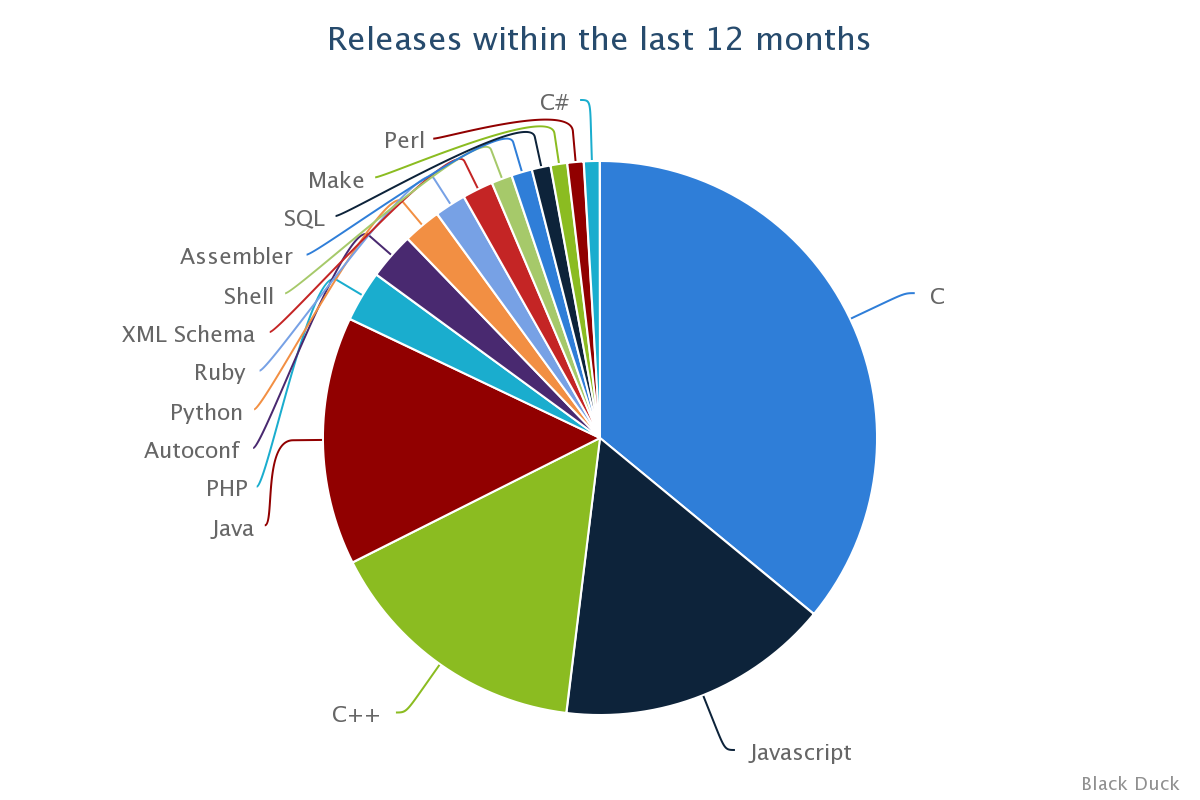
\includegraphics[width=0.9\linewidth]{../../data/js-trends/black-duck-15}

\paragraph{Jobs}

All these metrics are representing the visible activity about programming language.
But not the entire software industry is open source, and the activity is rather opaque.
To get a hint on the popularity of programming languages used in the software industry, let's look at the job offerings.
Indeed provide some insightful trends.
Javascript developers ranked at the third position, right after SQL developers and Java developers.
Then come C\# and C developers.

% TODO redo this graph, it is ugly.
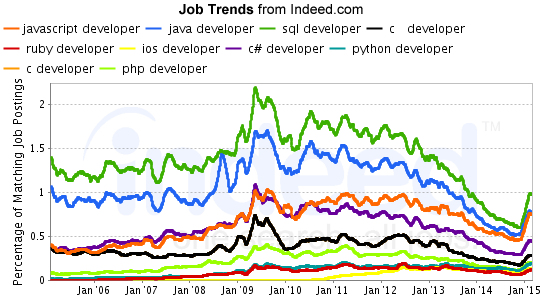
\includegraphics[width=0.9\linewidth]{../../data/js-trends/jobgraph}

All these metrics represent different faces of the current situation of Javascript adoption.
We can safely say that Javascript is one of most important language of this decade, along with Java, C/C++.
It is widely used in open source projects, and everywhere on the web.
But it is also trending, and maybe slowly replacing languages like Java.
% TODO continue this

\paragraph{Future trends}

\comment{TODO}

Code reuse.
Why it never worked ?




\comment{em-scripten}

https://github.com/kripken/emscripten
Javascript is a target language for LLVM, therefor everything can compile to Javascript : JS is the assembler of the web.

\comment{Isomorphic Javascript}

Server-side Javascript

https://www.meteor.com/
https://facebook.github.io/flux/
Javascript can be executed both on the client and the server.
That allow use-cases never possible before (server pre-rendering, same team ...)

\comment{Reactive}

http://facebook.github.io/react/
Javascript is used to model the flow of propagation of state in a web application



---

Some facts to include :
https://www.destroyallsoftware.com/talks/the-birth-and-death-of-javascript
The Atom editor is written in Javascript node.js.
Now, major PaaS (which one) support node.js by default.
Heroku support Python, Java, Ruby, Node.js, PHP, Clojure and Scala
Amazon Lambda Web service support node.js in priority.
npm raises 8m.
http://techcrunch.com/2015/04/14/popular-javascript-package-manager-npm-raises-8m-launches-private-modules/

% >>> I want to say that Javascript is now broadly used.
% Let's just look at the numbers : Javascript is the most popular language on Github, and npm has more package than any other package manager.
% Javascript has the more broadly deployed runtime.
% ... and so on
% >>> the conclusion is : Javascript is now a major language, and it is more than worth the consideration we are giving it in this PhD thesis.

\subsection{Overview of the language}

Javascript was released in a hurry, without a strong and directive philosophy.
During its evolution, it snowballed with different features to accommodate the community, and the usage it was made on the web. As a result Javascript contains various, and sometimes conflicting, programming paradigms.
It borrow its syntax from a procedural language, like C, and the object notation from an object-oriented language, like Java, but it provides a different inheritance mechanism, based on prototypes. Most of the implementation adopt an event-based paradigm, like the DOM\ftnt{http://www.w3.org/DOM/} and node.js\ftnt{https://nodejs.org/}.
And finally, event though it is not purely functional like Haskel, Javascript borrows some concepts from functional programming.

In this section, we focus on the last two programming paradigm, functional programming and event-based programming.
Javascript exposes two features from functional programming that are particularly adapted for event-based programming.
Namely, it treats functions as first-class citizen, and allows them to close on their defining context, to become closures.
% TODO In the next section, we explain this two features
% TODO and in the second section, we explain event-based programming and why these two features are good for event-based programming

\subsubsection{Functions as First-Class citizens}

\cit{All problems in computer science can be solved by another level of indirection}{Butler Lampson}

Javascript treats function as first-class citizens.
One can manipulate functions like any other type (number, string ...).
She can store functions in variables or object properties, pass functions as arguments to other functions, and write functions that return functions.

The most common usage examples of these features, are the methods \texttt{Map}, \texttt{Reduce} and \texttt{filter}.
In the example below, the method \texttt{map} expect a function to apply on all the element of an array to modify its content, and output a modified array.
A function expecting a function as a parameter is considered to be a higher-order function. \texttt{Map}, \texttt{Reduce} and \texttt{Filter} are higher-order functions.

\begin{code}
  [4, 8, 15, 16, 23, 42].map(function firstClassFunction(element) {
    return element + 1;
  });
  // -> [5, 9, 16, 16, 24, 43]
\end{code}

Higher-order functions provide a new level of indirection, allowing abstractions over functions.
To understand this new level of abstraction, let's briefly summarize the different abstractions on the execution flow offered by programming paradigms.
In imperative programming, the control structures allow to modify the control flow. That is, for example, to execute different instructions depending on the state of the program.
Procedural programming introduces procedures, or functions. That is the possibility to group instructions together to form functions.
They can be applied in different contexts, thus allowing a new abstraction over the execution flow.
% It encourages to abstract program states so that the same function can be applied in different places to apply its behavior.

So, higher-order functions add another level of abstraction.
It allows to dynamically modify the control of the execution flow.
The ability to manipulate functions like any other value allows to abstract over functions, and behavior.
% TODO continue this, there is a lot to say about HOF

Higher-order functions replace the needs for some Object oriented programming design patterns.\ftnt{http://stackoverflow.com/a/5797892/933670} Though object oriented programming doesn't exclude higher-order functions.

They are particularly interesting when the behavior of the program implies to react to inputs provided during the runtime, as we will see later.
Web servers, or graphical user interfaces, for examples, interact with external events of various types.

% TODO transition : higher-order functions makes use of closure to implement the lexical scope in mutable programming languages. (reformulate)

\subsubsection{Lexical Scoping}

Closures are indissociable from the concept of lexical environment.
To understand the former, it is important to understand the latter first.

\paragraph{Lexical environment}

A variable is the very first level of indirection provided by programming languages and mathematics.
It is is a binding between a name and a value.
Mutable like in imperative programming to represent the reality of memory cells, or immutable like in mathematics and functional programming.
These bindings are created and modified during the execution.
They form a context in which the execution takes place.
To compartmentalize the execution, a context is also compartmentalized.
A certain context can be accessed only by a precise portion of code.
Most languages defines the scope of this context using code blocks as boundaries.
That is known as lexical scoping, or static scoping.
The variables declared inside a block represent the lexical environment of this block.
These lexical environments are organized following the textual hierarchy of code blocks.
The context available from a certain block of code, that is set of accessible variable, is formed as a cascade of the current lexical environment and all the parent lexical environment, up to the global lexical environment.

% TODO draw the schema for a lexical environment here

\paragraph{Javascript lexical environment}
\ftnt{http://www.ecma-international.org/ecma-262/5.1/\#sec-10.2}

Javascript implement lexical scoping with function definitions as boundaries, instead of code blocks.
The code below show a simple example of lexical scoping in Javascript.

\begin{code}
  var a = 4;
  var c = 6;
  function f() {
    var b = 5;
    var c = 0;
    // a and b are accessible here.
    return a + b + c;
  }

  f(); // -> 9

  // b is not accessible here :
  a + b + c; // -> ReferenceError: b is not defined
\end{code}

Lexical scoping, or statical scoping, implies that the lexical environment are known statically, at compile time for example.
But Javascript is a dynamic language, it doesn't truly provide lexical scoping.
In Javascript, the lexical environments can be dynamically modified using two statements : \texttt{with} and \texttt{eval}.
We explain in details the Javascript lexical scope in section \ref{??? Compiler stuff}

\subsubsection{Closure}

\cit{An object is data with functions. A closure is a function with data.}{John D. Cook}

A closure is the association of a first-class function with its context.
When a function is passed as an argument to an higher-order function, she closes over its context to become a closure.
When a closure is called, it still has access to the context in which it was defined.
The code below show a simple example of a closure in Javascript.
The function \texttt{g} is defined inside the scope of \texttt{f}, so it has access to the variable \texttt{b}.
When \texttt{f} return \texttt{g} to be assigned in \texttt{h}, it becomes a closure.
The variable \texttt{h} holds a closure referencing the function \texttt{g}, as well as its context, containing the variable \texttt{b}.
The closure \texttt{h} has access to the variable \texttt{b} even outside the scope of the function \texttt{f}.

\begin{code}
  function f() {
    var b = 4;
    return function g(a) {
      return a + b;
    }
  }

  var h = f();
  // b is not accessible here :
  b; // -> ReferenceError: b is not defined

  // h is the function g with a closure over b :
  h(5) // -> 9
\end{code}


% TODO continue with closure


% TODO transition, Higher-order functions and closures are very handy in turn-based programming.
% Turn based programming is the programming model of the event-loop, which is the concurrent model for I/O bound applications.
% \section{Concurrency}


% http://berb.github.io/diploma-thesis/original/043_threadsevents.html

% On the Duality of Operating System Structures
% http://tolstenko.net/blog/dados/Unicamp/2010.1/mc714/extras/201_recomendada_Lauer-Needham-78-Duality.pdf

% Threads vs. Events
% http://courses.cs.vt.edu/cs5204/fall09-kafura/Presentations/Threads-VS-Events.pdf

% Why Threads Are A Bad Idea (for most purposes)
% http://www.cs.utah.edu/~regehr/research/ouster.pdf

% Why Events Are A Bad Idea (for high-concurrency servers)
% http://static.usenix.org/publications/library/proceedings/hotos03/tech/full_papers/vonbehren/vonbehren_html/

% http://www.usingcsp.com/cspbook.pdf

% Threads Without the Pain
% http://queue.acm.org/detail.cfm?id=1105678


% Cooperative Task Management without Manual Stack Management or, Event-driven Programming is Not the Opposite of Threaded Programming 
% http://static.usenix.org/publications/library/proceedings/usenix02/full_papers/adyahowell/adyahowell_html/

% Retrospective on SEDA
% http://matt-welsh.blogspot.fr/2010/07/retrospective-on-seda.html

% Latency
% http://highscalability.com/latency-everywhere-and-it-costs-you-sales-how-crush-it
% http://blog.gigaspaces.com/amazon-found-every-100ms-of-latency-cost-them-1-in-sales/




\subsection{About concurrent systems}

This demonstration focus on application depending on long waiting operations like I/O operations.
Particularly, this demonstration focus on real-time web services.
It is irrelevant for application heavily relying on CPU operations, like scientific applications.

Threads-based system and event-based system evolved significantly over the last half century.
These evolutions were fueled by the long-running debate about which design is better.
We try to succinctly and roughly retrace theses evolutions to understand the positions of each community.
This demonstration show that thread and events are two faces of the same reality.

Lauer and Needham \cite{Lauer1979} presented an equivalence between Procedure-oriented Systems and a Message-oriented Systems.

% TODO brief historic


Adya \textit{et. al.} analyzed this debate and presented fives categories through which to present the problem \cite{Adya2002}.
These two categories were often associated with thread-based systems and event-based systems.
% TODO not very clear
Their advantages and drawbacks were mistaken with those of thread and events.
Adya \textit{et. al.} explain in details two of these categories that are most representative, Task management and Stack management.
We paraphrase these explanations.

\subsubsection{Task management}

Consider a task as an encapsulation of part of the logic of a complete application.
All the task access the same shared state.
The Task management is the strategy chosen to arrange the task executions in available space and time.

Preemptive task management executes each task concurrently.
Their executions interleave on a single core, or overlap on multiple cores.
It allows to leverage the parallelism of modern architectures.
This parallelism has a cost however, developers are responsible for the synchronization of the shared memory.
While accessing a memory cell, it must be locked so that no other task can modify it.
Synchronization mechanism impose the developer to be especially aware of race condition, and deadlocks.
These synchronization problems make concurrency hard to program with preemptive task management.

The opposite approach, Serial task management, executes each task to completion before starting the next.
The exclusivity of execution assures an exclusive access on the memory.
Therefore, it removes the need for synchronization mechanism.
However, this approach is ill-fitted for modern applications, where concurrency is needed.

A compromise approach, Cooperative task management, allows tasks to yield voluntarily.
A task may yield to avoid monopolizing the core for too long.
Typically, it yields to avoid waiting on long I/O operations.
It merges the concurrency of the preemptive task management, and the exclusive memory access.
Thus, it relieves the developer from synchronization problems.
But at the cost of dropping parallel execution.

Threads are associated with preemptive task management, and events with Cooperative task management.
For this reason, it is commonly believed that synchronization mechanisms make threads hard to program \cite{Ousterhout1996}.
While it is really Preemptive task management that is responsible for these synchronization problems \cite{Adya2002}.

% TODO define the two
\subsubsection{Stack management}

Consider a task is composed of several subtasks interleaved with I/O operations.
Each I/O operation signal its completion with an event.
The task stops at each I/O operation, and must wait the event to continue the execution.
The stack management is the strategy chosen to express the sequentiality of the subtasks.

The automatic stack management is what is mostly used in imperative programming.
The execution seems to wait the end of the operations to continue with the next instruction.
The call stack is kept intact.
This is what is commonly called synchronous programming.

In the manual stack management, developers need to manually register the handlers to continue the execution after the operation.
The execution immediately continues with the next instruction, without waiting the completion of the operation.
It implies to rip the call stack in two functions; one to initiate the operation, and another to retrieve the result.
This is what is commonly called asynchronously programming.

% TODO advantage and disadvantages of synchronous and asynchronous programming

What we argue is that synchronous is good because it is linear, it avoids stack ripping.
But asynchronous is good because it allows parallelism by default.


% synchronous programming is good to express linear execution. In parallel that means quite unrelated linear executions.
% asynchronous programming is good to express interleaved parallel execution. It is easy to express small parallel and sequential tasks.


Threads are associated with the automatic stack management, and events with manual stack management.
For this reason, it is commonly believed that threads are easier to program.
\cite{Thread systems allow programmers to express control flow and encapsulate state in a more natural manner} \cite{Behren2003}.
However, the automatic stack management is not exclusive to threads.
Fibers, presented by Adya \textit{et. al.} is an example of cooperative task management with automatic stack management \cite{Adya2002} .
Fibers present the advantage of cooperative task management, without the disadvantage of stack ripping.
That is the ease of programming because of the absence of synchronization, without the difficulty of stack ripping.

We argue that the advantages of manual stack management outweigh its drawbacks for web services.
Because of the numerous I/O operations, parallelism is 


% TODO I split the explenation in thread then events, instead, I should split in task management, then state management




But what is actually highlighted is the automatic state management provided by threads.
And with lighter context change, threads are a good choice which provide parallelism.

Historically, events-based system are associated with manual state management, while threads-based systems are associated with automatic state management.
Manual state management imposed stack ripping \cite{Adya2002}.
With closure, it is not the case anymore.
Events now have automatic state management as well \cite{Krohn2007}.

Now, there is implementation of thread model with cooperative management, with context-switch overhead improved enough to fill the gap with events model.
And there is implementation of event model with automatic state management filling the gap with thread model.
In this condition, we ask, what really is the difference between thread and events.
We argue there is none.
Except the isolation, versus sharing of the memory, which, again is not significant of either.
In the first case, the different execution threads exchange messages, while in the second, they use synchronization mechanism to assure invariants in their states % TODO disambiguation thread is a context for execution, what is a core of execution ?

For a single thread of execution, both model could avoid synchronization through cooperative task management, which assure invariants. % TODO disambiguation
Or avoid procedure slicing (if any) using synchronization.
These are the two ends of a design spectrum.
One end (cooperative task management) fits better for small processing with heavy use of shared resources.
While the other end (synchronization) fits better for long processing with small use of shared resources.
When one end of the design spectrum is used while the other should be used, one might expect unresponsiveness because of too heavy events, or performance fall due to interlocking.

Scalability is achieved through parallelism, which is itself achieved in our case (web servers) through cluster of commodity machines.
% TODO this links exactly to what I wrote on scalability, find a way to merge the two.

With distribution, this design spectrum gets a better contrast. % TODO that is really false, reformulate to get a correct articulation

The synchronization of distributed, shared resources is limited through the CAP theorem  \cite{Gilbert2002a}. % TODO needs to read this.
Partition tolerance is a requirement of a distributed system. %TODO define PA, and find reference http://codahale.com/you-cant-sacrifice-partition-tolerance/#ft2
One needs to choose good latency (availability) or consistency. % Define the CAP theorem, consistency and availability
The CAP theorem is generalized into a broader theroem about\cite{Gilbert2012} % TODO read, and merge within the argumentation (the paper seems really broad, be careful not to dive too deep)

The isolation of resources implies to split the architecture in different stages, like Ninja \cite{Gribble2001}, SEDA \cite{Welsh2000}, or Flash \cite{Pai1999}.
This splitting is difficult for the developer.
The splitting which is good for the machine, is not the same as the one good for the design in modules.

The two ends of this design spectrum presented map directly onto the two kinds of parallelism advocated for scalability.
That is pipeline parallelism, and data parallelism.

Pipeline parallelism is good for data locality, and important throughput. % TODO reference
But each stage adds an overhead in latency. % TODO reference

Data parallelism is good for latency, because one request is processed from beginning to the end without waiting in queues.
But it implies that the different machines share a common database.
Which is a shared resource, and is limited by the CAP theorem.

Both parallelism have advantages and drawbacks, and both could be combined, like in the SEDA architecture. % TODO find the exact reference that says : it is good to use both parallelism to scale
Ultimately, it would be possible to design a design spectrum to choose which kind of parallelism for a set of requirements.
But we leave this for future works.

Splitting an architecture in stages is a difficult process, which prevent future code refactoring, and module modifications.
We argue that the design for the technical architecture, and the design for the human minds should not be the same.
Threads belong to the mental model, the design granularity
Events belong to the execution model, the architecture granularity
  % TODO quote
  It is a mistake to attempt high concurrency without help from the compiler \cite{Behren2003}.
Through compilation, we want to transform an event-loop based program (cooperative task management, no synchronization) into a pipeline parallelism distributed system.
So, basically, we argue that it is possible to distribute one loop event onto multiple execution core.



% TODO Careful, you don't know fibers enough.
% And globally, there is much that you don't know.

% Il y à quelques années, la tendance chez les gros était de se concentrer sur la parallélisation par threads pour gagner en latence.
% Notamment avec Gigaspace.
% Donc en occultant complètement les events, et en utilisant des grosses bases de données comme Dynamo ou Cassandra qui scalent bien.
% Je n'ai pas vraiment trouvé la même tendance pour les events.
% Storm et Spark stream sont à usage plus spécifique.
% Mais ce déséquilibre est peut être simplement dû à l'héritage de l'architecture n-tier.


% MICROSERVICES
% Plus récemment, j'ai trouvé beaucoup de bruit sur les microservices en 2014.
% Ça me paraissait intéressant, en pensant y trouver des arguments pour favoriser les events, et nuancer la tendance précédente.
% Mais j'ai l'impression qu'il s'agit plus d'une question d'organisation humaine que de performance.
% Il me reste à trouver des arguments pour mettre à égalité les deux axes de parallélisation.





% TODO 
% Continue with the hybrid approach : multiple threads for events, and one threads for user code
% See Flash, SEDA, Node.js etc ...






/!\ WARNING
The paper Why events are a bad idea states that :
the control flow patterns used by these applications fell into three simple categories: call/return, parallel calls, and pipelines.
Indeed, it is no coincidence that common event patterns map cleanly onto the call/return mechanism of threads. Robust systems need acknowledgements for error handling, for storage deallocation, and for cleanup; thus, they need a “return” even in the event model.
>> Why is it completly false ?
	 It is crucial to find an answer.
Moreover, Ayda et. al. state that :
For the classes of applications we reference here [file servers and web servers], processing is often partitioned into stages.
Other system designers advocated non-threaded programming models because they observe that for a certain class of high-performance systems [...] substantial performance improvements can be optained by reducing context switching and carefully implementing application-specific cache-conscious task scheduling.


The paper Why events are a bad idea states that :
One could argue that instead of switching to thread systems, we should build tools or languages that address the problems with event systems (i.e., reply matching, live state management, and shared state management). However, such tools would effectively duplicate the syntax and run-time behavior of threads.
>> Well, yes ...
   With the exception of the stack junction.
   The paper on Duality had it right, their graph is correct, but for threads, it cannot be distributed because of stacks, while for events, it can.


Software evolution substantially magnifies the problem of function ripping: when a function evolves from being compute-only to potentially yielding, all functions, along every path from the function whose concurrency semantics have changed to the root of the call graph may potentially have to be ripped in two. (More precisely, all functions up a branch of the call graph will have to be ripped until a function is encountered that already makes its call in continuation-passing form.) We call this phenomenon ``stack ripping'' and see it as the primary drawback to manual stack management. Note that, as with all global evolutions, functions on the call graph may be maintained by different parties, making the change difficult. 
>> Stack ripping is what I am talking about.
   While the stack are joined, it is not possible to distribute.
   If they say that stack ripping is necessary, that means it is not possible to encapsulate asynchronous function into synchronous function.
% \section{Scalability}

% TODO introduction to this chapter


We define a web service as a computer program whose main interface is based on web protocols, such as HTTP.
Such a service uses resources allocated on a network of computers.
Scalability defines the ability of the service to use a certain quantity of resource to meet a desired performance.
We call system the association of the computer program and the available resources. 
The performance of this system is measured by its latency and throughput.

\subsection{Latency and throughput}

Latency is the time elapsed between the reception of a request, and the sent of the reply.
It includes the time waiting for resources to be free to process the request, and the time to process the request.

Throughput is the number of requests processed by the system by unit of time.

Latency and throughput are linked in a certain way.
If a modification of the web service reduces its mean latency to a half, then the throughput doubles immediately.
It takes half the time to process a request, therefore, the service can process more requests in the same time.
However, if throughput augment, the latency doesn't necessarily decrease.

\subsection{Scalability granularity}

We define a computer program as a set of operations.
In the case of a web service, these operations can be directly requested by the user through the interface.
An operation can cause any other operation to execute.

Because both the resources used and the operations executed are discrete : not infinitely divisible, scalability is inherently discrete.


% TODO scalability granularity ? 
Scalability granularity is the increment of resources.
How the input data can be split up ?
How the program can be deployed on many machines ?






We call system the association of the computer program with the resources


\subsection{Horizontal and vertical scaling}

There is two ways to augment the resources of the system.
Enhance the nodes in the computer network - vertical scaling.
Or add more nodes to the computer network - horizontal scaling.


% TODO how to apply these theory to highly concurrent servers ?
% How does it modify the theories ?

There are three theories, from the most restrictive, to the most general.


% TODO define scalability
Scalability is the property of a computer program to occupy available resources to meet a needed performance.
EIther in Latency, or in throughput.







\subsection{Linear scalability}

Clements et. al. \cite{Clements2013a} prove that a computer program scale linearly if all its operations are commutative.
% Commutative is not parallel. How to go from commutative to parallel ?
Two operations are said to be commutative if they can be executed in any orders, and the same initial state will result in the same final state.
Commutativity implies the two operations to be memory-conflict free, or independent, which is equivalent to say that they can be executed in parallel.

Therefore, to achieve linear scalability, a computer program must be composed of a set of operations that commutes.
Thus, all the operations are parallel, they can be executed simultaneously, on any number of machines as required.

The size of the operations sets the scalability granularity.

However, commutativity is not achievable in real applications.
Even sv6, the operating system resulting from the work on commutative scalability only has 99\% commutativity.
For real application, in the best case, the granularity is coarse, in the worst case, there is no possible commutativity because of shared resources (like a product inventory, or a friend graph).

% TODO continue

\subsection{Limited scalability}

Amdahl introduced in 1967 a law to predict the limitation of speedup a computer program can achieve if a fraction of its code is sequential.
Amdahl worked at increasing the speed of computer clock, while the scientific community was working on improving parallelism of computing machines.

In a set of operations, even if one is non-commutative, it cannot be executed in parallel of any others, the scalability is limited by this operation.

There is a difference if the operation is non-commutative with itself, or only with others.
In the first case, it impose a queuing, while in the second case, it only increase the granularity : you can regroup the non-commutative operation with its subsequents, and form a bigger commutative operation.

% TODO continue

\subsection{Negative scalability}

Gunther generalized Amdahl's law into the Universal Scalability Law.
It includes the parallelization of non-independent operations with the use of synchronization.

It models the negative return on scalability from sharing resources observed in many real world applications.

% TODO continue by explaining the different area of scalability.



\subsection{Eventual Consistency}

To overpass the scalability limits set by the previous rules, it is possible to abandon consistency.
It simply tolerate incoherences between multiple replicas.
The output of an operation can be false while its state is synchronized with the other replicas.

% It is similar to the propagation of sound, light or gravity.
% When an explosion happens, not everybody hears it at the same time : there is inconsistency in the experience.


% TODO continue

% \section{Framworks for web application distribution}
% \subsection{Micro-batch processing}
% \subsection{Stream Processing}

% \section{Flow programming}
% \subsection{Functional reactive programming}
% \subsection{Flow-Based programming}

% \section{Parallelizing compilers}
% \comment{OpenMP and so on}
% %\subsubsection{\comment{TODO}}

% \section{\comment{Synthesis}}
% \comment{There is no compiler focusing on event-loop based applications}


%-----------------------------------------------------------------------------%
                                    \endinput
%-----------------------------------------------------------------------------%

Objective
---------

My objective is to find a solution to allow a first code base to evolve continuously in performance. That is to avoid the rupture that is so often observed in the industry currently (e.g. LinkedIn, Facebook ... ).

I want to achieve that with a solution to transition from the imperative model presenting certain characteristics to a distributed model with certain conditions.

Cartography
-----------


# Industry -> We want to decrease development time while increasing performance. We barely care about used resources.

## Languages, libraries and frameworks

  + Java - Object-oriented
  +> Spring
  +> Scala - Functional + Object-oriented
  +>> Akka - Message driven actors
  +>>> Play - on top of akka (Asynchronous)

  + PHP - Object-oriented
  +> Sinatra

  + Ruby - Functional + Object-oriented
  +> Rails

  + Javascript - Functional + Prototype-oriented
  +> Express.js
  +> hapi.js
  +> Meteor
  +> Bacon.js - Reactive programming
  +> kraken.js

  + NoFlo

  + Haskell
  +> FRP Reactive programming

  + Spidle: A DSL approach to specifying streaming applications dataflow like

  + Erlang

## Databases

  + FlockDB
  + CouchDB
  + PouchDB
  + Cassendra
  + Dynamo DB

  + unhosted
  + MoveMyData

## Runtime

  + Node.js - Asynchronous programming with Event-loop
  +> Fibers 


# Embedded -> We want to decrease used resources while increasing performance. We barely care about development time.



+ Exploiting Coarse-grained Task, Data and Pipeline Parallelism in Stream Programs -> Compile StreamIt to assembler for multi-core

+ Shangri-La - Compile C-like into assembler for packet program

+ SPUR - A programming model for an embedded media processing architecture


# Scientific-like -> We want to increase performance. We barely care about used resources nor decreasing development time.

## Languages, libraries and frameworks

  + OpenMP
  + OpenCL
  + CUDA
  + Cg: A system for programming graphics hardware in a C-like language
  + Brook for GPUs: Stream Computing on Graphics Hardware
  + Liquid Metal by IBM - unified language for FPGAs, GPUs and such ...

  + StreaMIT: A language for Streaming Applications


  + Apache Kafka - publish/subscribe distributed commit log

  Design methodology:
  + PCAM - Partition -> Communicate -> Agglomerate -> Map

## Runtime

  + Vert.X - node like + thread / worker capabilities

  OSs :

  + BarrelFish
  + TesselationOS
  + Mosix
  + CoreOS


  Architectures:


    Web service oriented:
      Threads only:
      + Capricio - User cooperative threads (also known as fibers / green threads)

      Events only:
      + TAME - event-based solution without stack ripping in C (it is like closure, but for C)

      Hybrid solutions:
    + AMPED Asymetric multi-process event-driven
    +> Flash
    +> Nginx
    +> Ninja
    +> SEDA
    +> Leda - PCAM 
    + Combining events and threads for scalable network services, Linguistic symbiosis between event loop actors and threads, Combining data flow and control flow computing)

    + 

    + Cluster-based scalable network services


  + Grape / Timestream - distributed SQL (roughly)
  + CQL
  +> STREAM (uses CQL)
  + StreaQuel
  +> TelegraphCQ
  + AQuery

  (From the paper : Making state explicit for imperative big data processing)
  + MapReduce       map/reduce   |   Stateless dataflow
  + DryadLINQ       functional   |   Stateless dataflow
  + Spark           functional   |   Stateless dataflow
  + CIEL            imperative   |   Stateless dataflow
  + Hadoop          map/reduce   |   Stateless dataflow
  + Incoop          map/reduce   |   Incremental dataflow
  + Nectar          functional   |   Incremental dataflow
  + CBP             dataflow     |   Incremental dataflow
  + Comet           functional   |   Batched dataflow
  + D-Streams       functional   |   Batched dataflow
  + Naiad           Dataflow     |   Batched dataflow
  + Storm, S4       dataflow     |   Continuous dataflow
  + SEEP            dataflow     |   Continuous dataflow
  + Piccolo         imperative   |   Parallel in-memory
  + SDG             imperative   |   Stateful dataflow




What about all the techniques for analyzing and extracting parallelism :

+ Commutativity analysis: a new analysis technique for parallelizing compilers
+ the scalable commutativity rule ...
+ Making asynchronous parallelism safe for the world


+ Cooperative task management without manual stack management - Hybrid approach, fibers + threads




- transactional memory
  - http://www.morganclaypool.com/doi/abs/10.2200/s00272ed1v01y201006cac011
  - http://delivery.acm.org/10.1145/1370000/1364800/p80-larus.pdf?ip=160.92.8.31&id=1364800&acc=OPEN&key=4D4702B0C3E38B35.4D4702B0C3E38B35.4D4702B0C3E38B35.6D218144511F3437&CFID=529578904&CFTOKEN=25104956&__acm__=1437488908_6eeb5d92ab07593b1aa92d3ac4461c0b
  - ...

- Continuation-passing style parallelization
  - The interprocedural analysis and automatic parallelization of Scheme programs - http://link.springer.com/article/10.1007/BF01808954#page-1
  - 

- Event-loop / 




Criteria
--------






\section{Seamless Development} \label{chapter3:objectives}
\nt{TODO title not clear enough}

\begin{center}
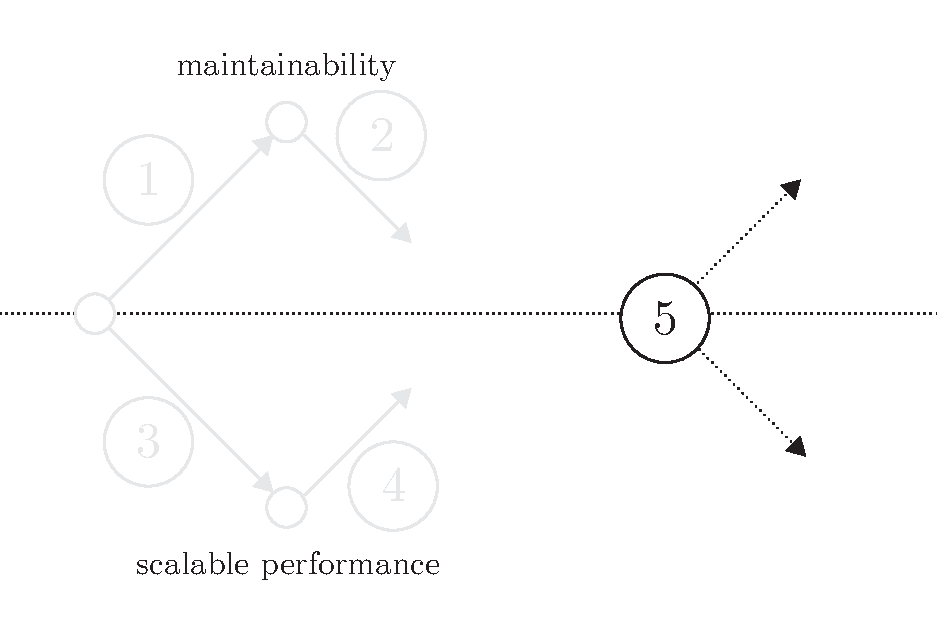
\includegraphics[width=0.6\textwidth]{../ressources/state-of-the-art-5.pdf}
\end{center}

The section \ref{chapter3:software-maintainability} shows that the modular organization enabled by functional programming is the best way to improve maintainability.
But it requires the use of a global memory store which conflicts with performance.
Compilation is a solution to reduce this conflict, but is not yet satisfactory enough for high performance scalability.
On the other hand, the section \ref{chapter3:software-performance} shows that to attain performance scalability, an application needs to multiply the exclusive accesses to its state.
That implies follow a distributed organization of its state to provide isolation and immutability, which negatively impacts modularity, hence maintainability.
Some works provide a uniform memory access to improve maintainability, despite the distributed execution.

The evolution of the economical constraints of a web application requires to repeatedly switch between maintainability and performance scalability.
The incompatibility between the two organizations implies technological ruptures at each switch.
Huge developing efforts are pulled to translate manually from one organization into the other, and later to maintain the implementation despites its unmaintainable nature.
There is still room for improvements on a compromise between maintainability and performance scalability.

The state of the art highlighted that
\begin{itemize}
\item maintainability requires lazy-evaluation and higher-order programming, section \ref{chapter3:software-maintainability:programming-models:functional-programming}, and
\item higher-order programming requires a global memory abstraction, section \ref{chapter3:software-maintainability:modular-programming:limitations},
\end{itemize}
Javascript is a functional language that features higher-order programming and a global memory abstraction.
% Moreover, its dynamic natures allows a lot of flexibility for the developers.
Moreover, node.js features a streaming approach with the event-loop execution model, similar to the lazy evaluation.
These reasons make Javascript a language of choice for developing web application.

And that
\begin{itemize}
\item scalable performance requires parallelism, and
\item parallelism requires exclusive accesses on the state through isolation and immutability.
\end{itemize}
Eventually, web development is heading toward a streaming approach with pipeline processing.

\nt{TODO dependency schema of these highlights}

This thesis proposes an equivalence between the global memory and control flow on one hand, and memory isolation with message passing on the other hand.
It proposes this equivalence as a solution to conciliate the scalable performance and maintainability.
As explained below, the concurrency model of the event-loop execution model, and the parallel approach of the pipeline execution model are very similar.
The goal of this thesis is to allow to compile one execution model into the other, to allow developers to constantly keep two organization of their implementation, allowing them to focus on both maintainability and scalable performance.

\subsection{Equivalence}

The next paragraphs introduces this equivalence between the event-loop execution model and the pipeline execution model.
The equivalence addresses two \textit{levels}\nt{not the good word}, as illustrated in figure \ref{fig:chapter3:objectives:roadmap}, the control flow, and the memory isolation.

\begin{figure}[h!]
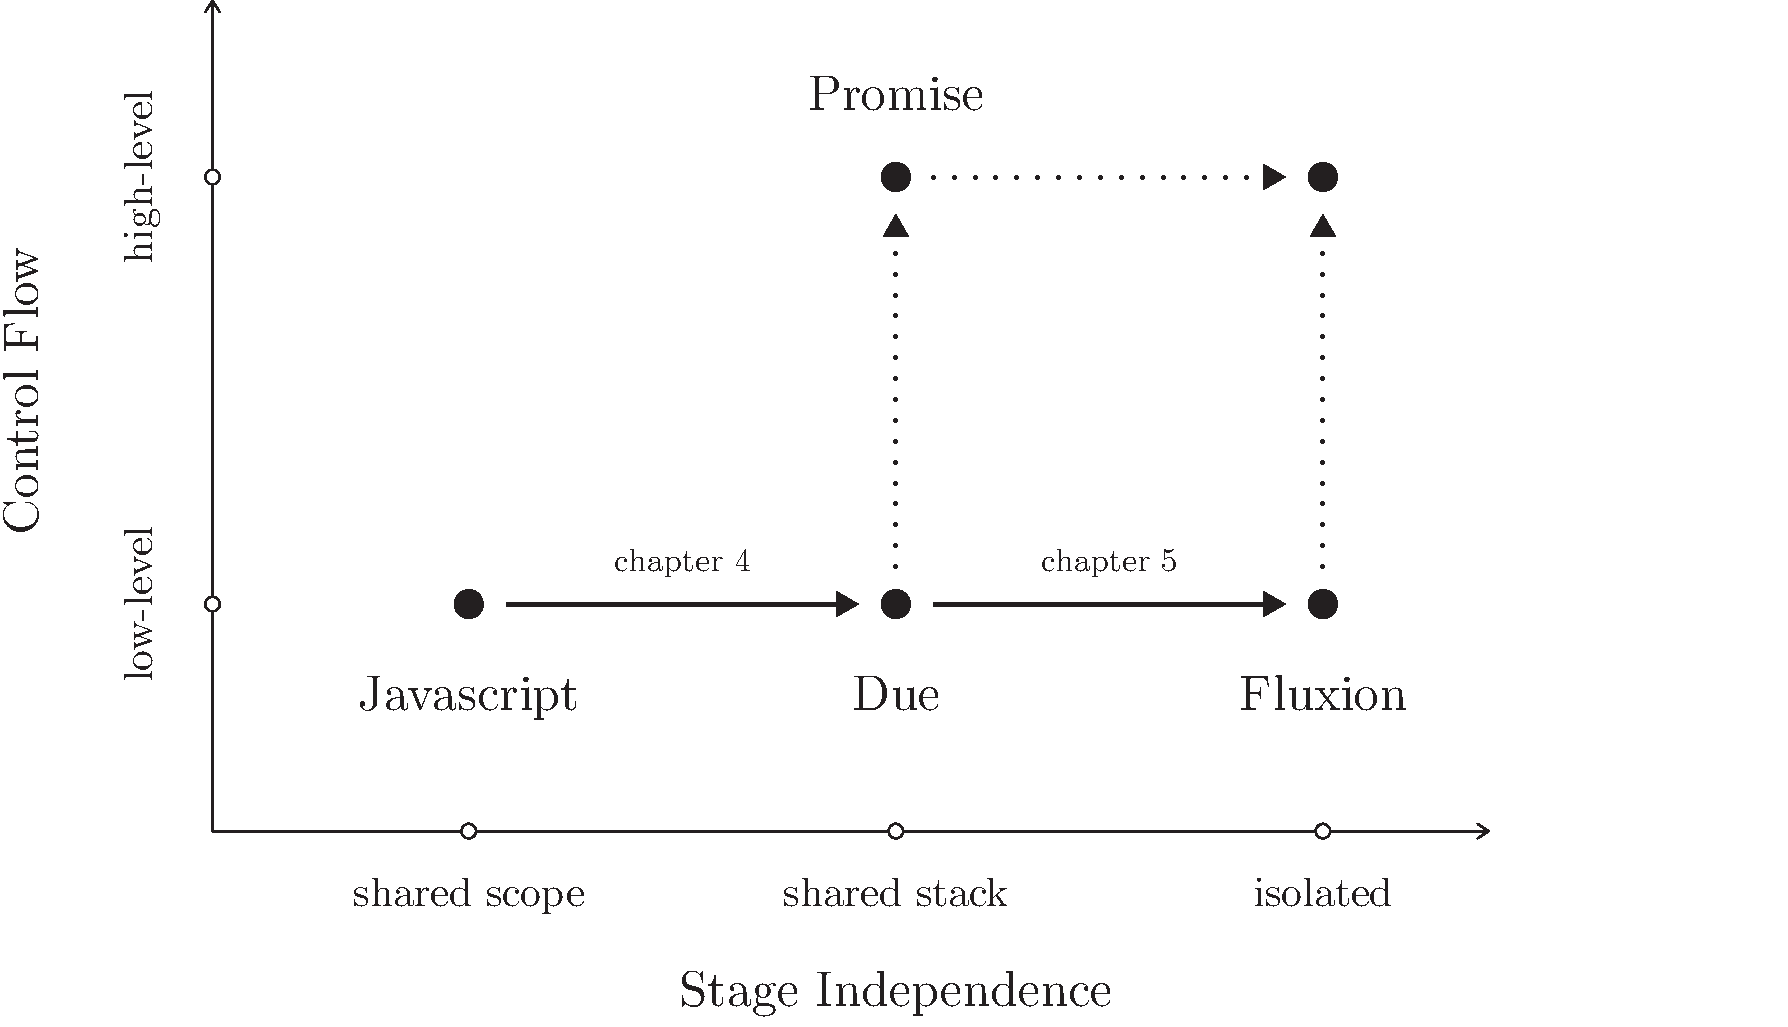
\includegraphics[width=1\textwidth]{../ressources/roadmap.pdf}
\caption{Roadmap}
\label{fig:chapter3:objectives:roadmap}
\end{figure}

\subsubsection{Rupture Point}

The execution of the pipeline architecture is well delimited in isolated stages.
Each stage has its own thread of execution, and is independent from the others.
On the contrary, the code of the event-loop is linear because of the continuation passing style and the common memory store.
% The message passing linking the callbacks is transparently handled by the event-loop.
However, the execution of the different callbacks are as distinct as the execution of the different stages of a pipeline.
The call stacks of two callbacks are distinct.
Therefore, an asynchronous function call represents the rupture between two call stacks.
It is a rupture point, and is equivalent to a data stream between two stages in the pipeline architecture.

Both the pipeline architecture and the event-loop present these rupture points.
The detection of rupture points allows to map a pipeline architecture onto the implementation following the event-loop model.
To allow the transformation from one to the other, this thesis studies the possibility to detect rupture points, and to distribute the global memory into the parts defined by these rupture points.
The detection of rupture points is addressed in chapter \ref{chapter4}.

It presents the extraction of a pipeline of operations from a Javascript application.
Indeed, such pipeline is similar to the one exposed by Promises.
The chapter proposes a simpler alternative to the latter called Dues.
However, these operations still require a global memory for coordination so they are not executed in parallel.

\subsubsection{Invariance}

% This transformation is important on two points.
% The conservation of the invariance.
% The equivalence between the coordinations.

The transformation should preserve the invariance as expressed by the developer to assure the correctness of the execution.
The partial ordering of events in a system, by opposition to total ordering, is sufficient to assure this correctness.
% This result was used by Lamport to prove the correctness of distributed systems.
The global memory is a way to assure the total ordering of events, and the message passing coordination is a way to assure partial ordering of events.
Therefore, to assure the correctness of the execution of a system, the state coordination with a global memory is equivalent to message passing coordination.
And it is possible, at least for some rupture points, to transform the global memory coordination into message passing while conserving the correctness of execution.

In order to preserve the invariance assured by the event-loop model after the transformation, each stage of the pipeline needs to have an exclusive access to memory.
The global memory needs not to be split into parts and distributed into each of the stages.
To assure the missing coordinations assured by the shared memory between the stages, the transformation should provide equivalent coordination with message passing.
The isolation and replacement of the global memory is fully address in chapter \ref{chapter5}, with the introduction of isolated containers called Fluxions.




% The invariance holds for the whole memory during the execution of each callback.
% As I explained in the previous section, this invariance is required to allow the concurrent execution of the different tasks.
% On the other hand, the invariance is explicit in the pipeline architecture, as all the stages have isolated memories.
% The coordination between these isolated process is made explicit by the developer through message passing.

% I argue that the state coordination between the callbacks requireing a global memory could be replaced by the message passing coordination used manually in the pipeline architecture.
% I argue that not all applications need concurrent access on the state, and therefore, need a shared memory.
% % Specifically, I argue that each state region remains roughly local to a stage during its modification.
% \nt{TODO review that, I don't know how to formulate these paragraphs. Identify the state and the data in the global memory.}

% \subsubsection{Transformation}

% This equivalence should allow the transformation of an event loop into several parallel processes communicating by messages.
% In this thesis, I study the static transformation of a program, but the equivalence should also hold for a dynamic transformation.
% I present the analyzis tools I developed to identify the state and the data from the global memory.



TODO Talk about the annotations used by many parallel languages.



Some links I NEED to put :
--------------------------

https://glyph.twistedmatrix.com/2014/02/unyielding.html
http://calculist.org/blog/2011/12/14/why-coroutines-wont-work-on-the-web/

Transitions :
  - Linkedin - http://engineering.linkedin.com/architecture/brief-history-scaling-linkedin
  - Facebook - https://www.cs.princeton.edu/events/event/evolution-software-architecture-facebook / http://www.infoq.com/presentations/Evolution-of-Code-Design-at-Facebook
  - ... 

https://medium.com/@benorama/the-evolution-of-software-architecture-bd6ea674c477

https://en.wikipedia.org/wiki/Dataflow
https://en.wikipedia.org/wiki/Real-time_computing
https://en.wikipedia.org/wiki/Partitioned_global_address_space
https://en.wikipedia.org/wiki/SPMD

Albert Cohen
https://scholar.google.com/citations?user=MkKZKAMAAAAJ&hl=en

+ Paul Feautrier (Tutor of A. Cohen)


SPMD Single program multiple data
Partitioned global address space


Some chunks I might find useful later :
---------------------------------------

\cit{No matter how great the talent or efforts, some things just take time. You can't produce a baby in one month by getting nine women pregnant.}
{Warren Buffett}

A good example of declarative sentence in everyday world : in case of fire, 
the elevators don't work -> you understand that you need to take the stairs.

The purpose of explicit synchronization is to manage the timing of side-effects in the presence of parallelism. 

A function is side-effect free if it is referentially transparent.



---


We presented in the introduction the popularity of Javascript, we argue that using this position to leverage parallelism is the only solution, and that proposing a new language, only on the base that it provide parallelism could not possibly make this language popular and grow a community.

Therefore, the only solution is to use the existing languages as is, and to compile them to gain parallelism.